\documentclass[12pt]{article}
%%%%%%%%%%%%%%%%%%%%%%%%%%%%%%%%%%%%%%%%

\usepackage{barddoc}

\title{The \bard package
       \thanks{This file has version number \barvers and describes \bard ver.\barvers}
}


\makeindex

%%%%%%%%%%%%%%%%%%%%%%%%%%%%%%%%%%%%%%%%
\begin{document}
\maketitle
\begin{abstract}
The \bard package is inspired and entirely based on \pst package.
The main purpose is to make the drawing of (simple) 
bar diagrams possible and (I hope) easy  in La\TeX{}.  
\end{abstract}

%%%%%%%%%%%%%%%%%%%%%%%%%%%%%%%%%%%%%%%%%%

\mysection{Package installation \label{sec:1}}

The \bard package consists of two sty-files: 
\pac{bardiag.sty} (written by me)
and \pac{pstfp.sty} which is an almost exact copy of 
the \pac{fp-basic.sty} package
by Michael Mehlich. The second one is needed to work with floating
point numbers and has been patched to work with \pac{multido.sty} from the
\pst. The \pac{bardiag.sty} also loads \pac{bardiag.bar} with some 
internal routines.

The \bard depends on \pac{pstricks}, \pac{pstcol}, \pac{pst-grad},
\pac{multido}, \pac{calc}, \pac{fp-snap}, \pac{ifthen}, 
so make sure they are installed. Then copy 
the \pac{bardiag.sty}, \pac{bardiag.bar}, and \pac{pstfp.sty} 
files into your texmf tree,
where La\TeX{} is able to find them. That's it!

This manual consists of three files: this one (\texttt{bardiag.ps}), 
\texttt{bardiag1.ps}, and \texttt{bardiag2.ps}.
The present one describes the installation and features needed to draw
``vertically'' oriented diagrams, i.e. with bars parallel to 
the Y-axis; \texttt{bardiag1.ps}  explains how to build ``horizontal''
bar diagrams; and \texttt{bardiag2.ps} includes all appendices,
including some source listings and examples of alternative shapes, not
included in the \bard\texttt style-file itself, but available as a config file.

In the \pac{example} directory you can find: (i) \pac{diagrams.tex} which
contains some examples of colored diagrams; (ii) \pac{diagramsbw.tex} with b/w
diagrams -- it is shown how to use pattern filling instead of color; (iii)
\pac{altdiags.tex} represents some ``alternative'' bar shapes.

\mysection{Quick start \label{sec:2}}

\subsection{Simple bar diagram \label{sec:2.1}}
Let me start from an example. One wants to draw a diagram, representing table~\ref{tab:1}.
\begin{table}[!h]\centering
\begin{tabular}{c||ccccc}
Year    & 1998 & 1999 & 2000 & 2001 & 2002 \\\hline
Income  & 120  & 123  & 147  & 176  & 132
\end{tabular}
\caption{\label{tab:1} See diagram \figref{fig:1}.}
\end{table}
%  
It can be done with the following piece of code
\lstinputlisting{figs/examp1.tex}
The result is \figref{fig:1}. 
So, a bit of explanation now.

Any diagram begins with \verb+\bardiagrambegin+ 
\index{Commands!bardiagrambegin}
and ends with
\verb+\bardiagramend+ \index{Commands!bardiagramend}
commands. Arguments of the first one are\\
\verb+\bardiagrambegin{diagheight}{diagwidth}{bottomheight}{dbar}{dx}{xunit}{yunit}+

\begin{figure}[t]\centering
  \input{figs/examp1.tex}
\caption{\label{fig:1} Example 1 to table~\ref{tab:1}.}
\end{figure}

\begin{figure}[t]\centering
  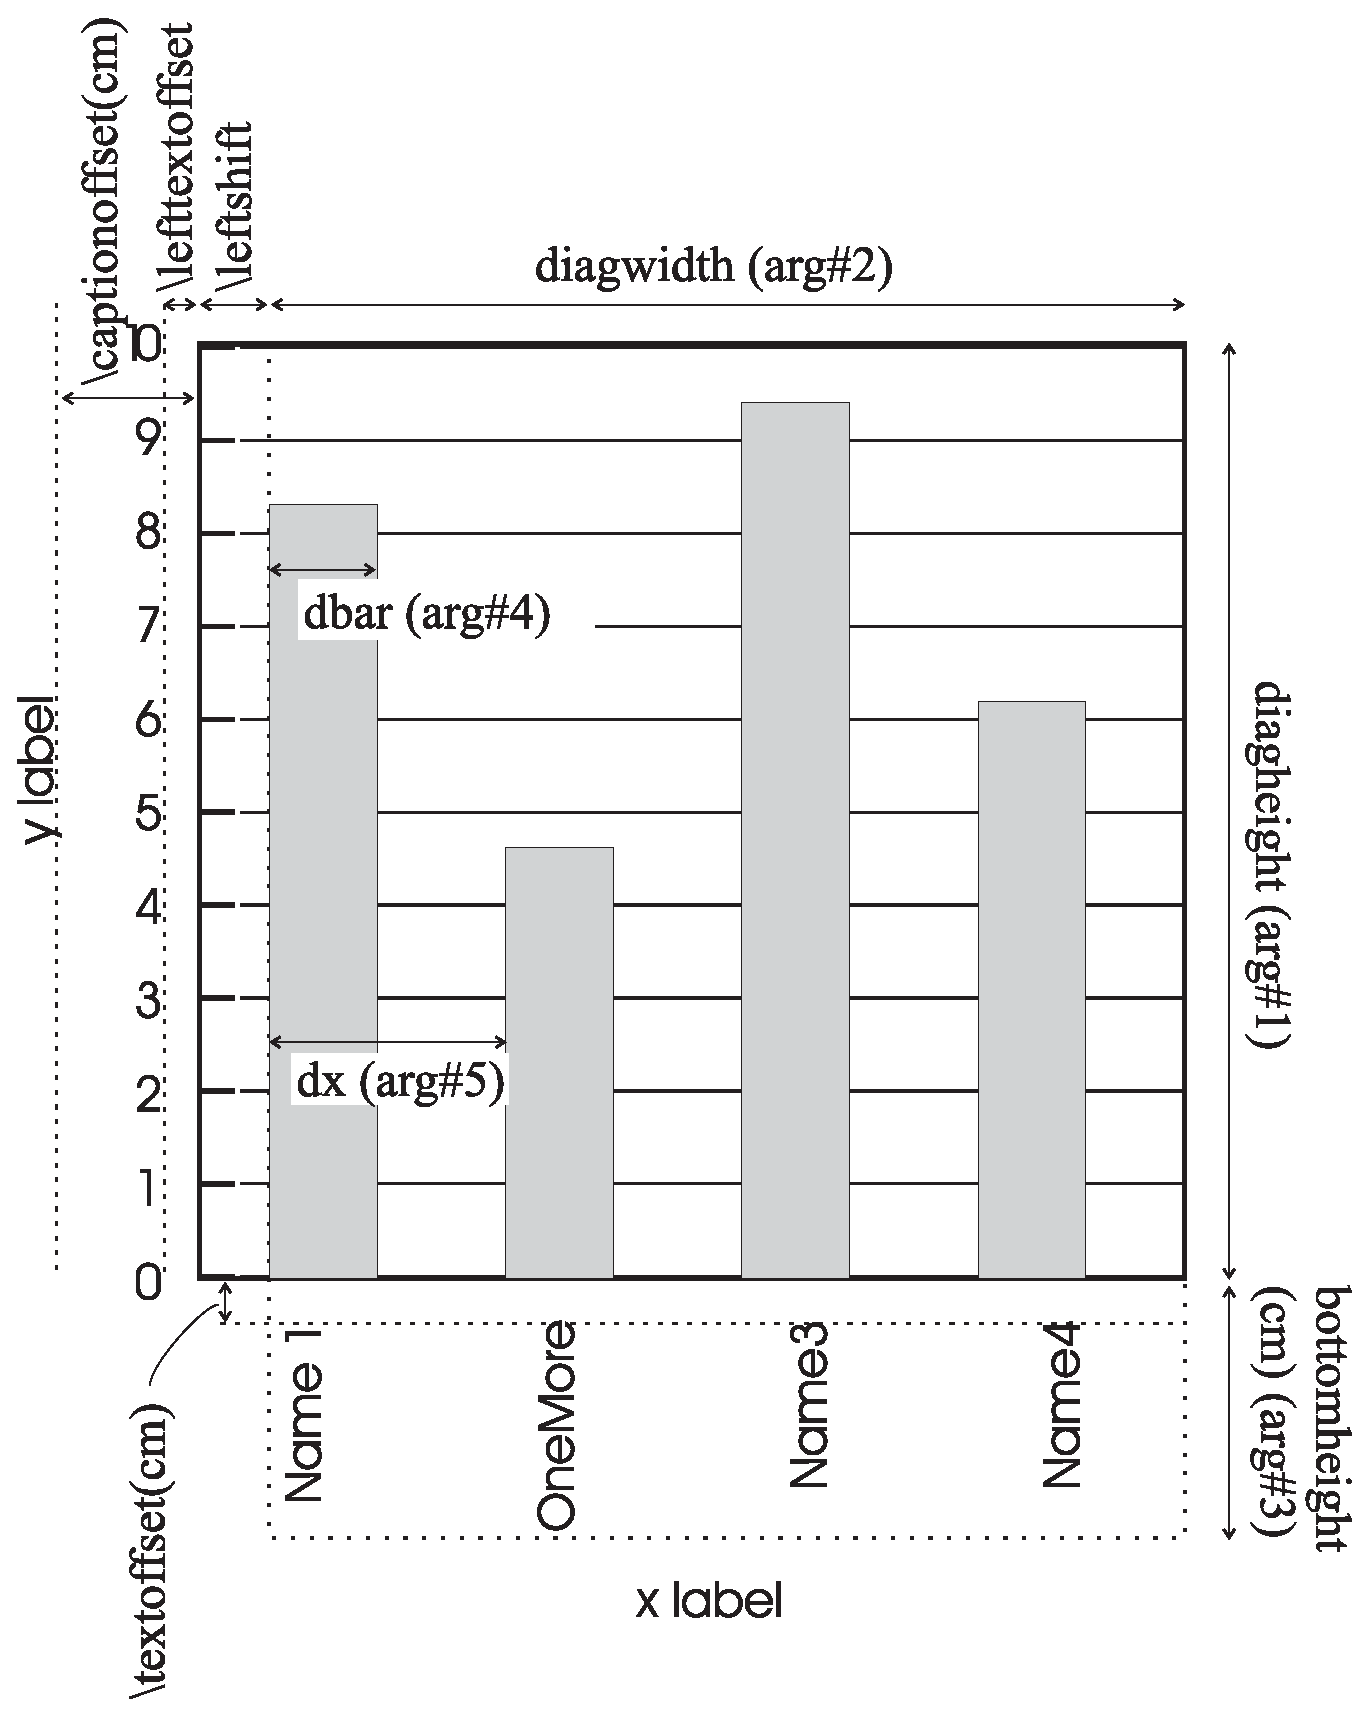
\includegraphics[scale=0.5]{figs/diag.eps}
  \caption{\label{fig:2} Arguments (shown with \#1..5) of the
    \texttt{bardiagrambegin} command and other parameters}
\end{figure}

The meaning of the first 5 arguments is apparent from the
\figref{fig:2}. The 6th and the 7th parameters are unit lengths along
x- and y-axis correspondingly. Note, that \texttt{diagheight},
\texttt{diagwidth}, \texttt{dbar}, and \texttt{dx} are NOT lengths, but
(floating point) numbers. They are then converted to lengths
automatically using \texttt{xunit} and \texttt{yunit}. However
\texttt{bottomheight} is a ``real'' length and should be accompanied,
exactly as \texttt{xunit} and \texttt{yunit}, by \texttt{cm} or
\texttt{in} or whatever you find more comfortable for yourself. This
allows to scale the diagram changing \texttt{xunit} and/or
\texttt{yunit} but leave the bottom part of the same height. Just to
demonstrate that I drew the same diagram
 as \figref{fig:1}, but used a
smaller last argument in \texttt{bardiagrambegin}:\\
\verb+\bardiagrambegin{9.5}{200}{2cm}{1}{2}{1cm}{0.01cm}+\\
As you see on \figref{fig:3} the bottom remains readable.
\begin{figure}[!ht]\centering
  \renewcommand{\betweenticks}{50}
\bardiagrambegin{9.5}{200}{2cm}{1}{2}{1cm}{0.01cm}
    \drawlevellines
    \baritem{1998}{120}{green}
    \baritem{1999}{123}{red}
    \baritem{2000}{147}{yellow}
    \baritem{2001}{176}{green}
    \baritem{2002}{132}{red}  
\bardiagramend{{\large Year}}{{\large Income}}

\caption{\label{fig:3} The same data as in \figref{fig:1} but 
          \texttt{yunit} is 0.1cm instead of 0.5cm.}
\end{figure}

The \verb+\bardiagrambegin+ begins a bar diagram and 
\verb+\bardigramend+ \index{Commands!bardiagramend}
ends it. It has two arguments: x and y label. In
the example above they are \verb+{\large Year}+ and 
\verb+{\large Income}+ correspondingly. 

Between the ``begin'' and ``end'' statements
one actually ``draws the stuff''. Command\\ 
\verb+\baritem{caption}{value}{color}+ \index{Commands!baritem}
Draws a bar of height \texttt{value} using color \texttt{color} and
prints \texttt{caption} below it. By default it also prints numbers
\index{Numbers}
(values) near the top of the bar - how to change this behavior is
explained further on [section~\ref{sec:3.3}].

Command \verb+\drawlevellines+ draws horizontal lines and put ticks
with numbers along the y-axis. An important parameter in this case is
the \verb+\betweenticks+ \index{Parameters!betweenticks}. It
determines the distance between ticks (level lines) in units of
\texttt{yunit}. Note that the \verb+\drawlevellines+ can be issued at
any point inside the diagram. In this way bars can lie over (as in
\figref{fig:1}) or be behind the level lines.
      
\subsection{Adding a legend \label{sec:2.2}}
The next step is to add a legend to the diagram: 
\lstinputlisting{figs/examp1b.tex}
The result is shown in \figref{fig:4}.
\begin{figure}[t]\centering
  \input{figs/examp1b.tex}
\caption{\label{fig:4} Adding legend to \figref{fig:1}}
\end{figure}

Any legend begins with 
\verb+\diagLegendbegin{Xupleft}{Yupleft}{width}+,
\index{Commands!Legend!diaglegendbegin}
where the first two arguments represent the upper left point of the
legend's bounding box (see \figref{fig:5}) and the last one its width.
The height of the box is  calculated automatically.

\verb+\diagLegenditem{caption}{icolor}+ produces a rectangle of the
color \texttt{icolor} and prints \texttt{caption} next to it. To finish
the legend the \verb+\diagLegendend+
\index{Commands!Legend!diagLegendend}
is used. Note, that \emph{all} these coordinates are in \texttt{xunit}
and \texttt{yunit} units, not in \texttt{cm} or \texttt{in}!
\begin{figure}[t]\centering
  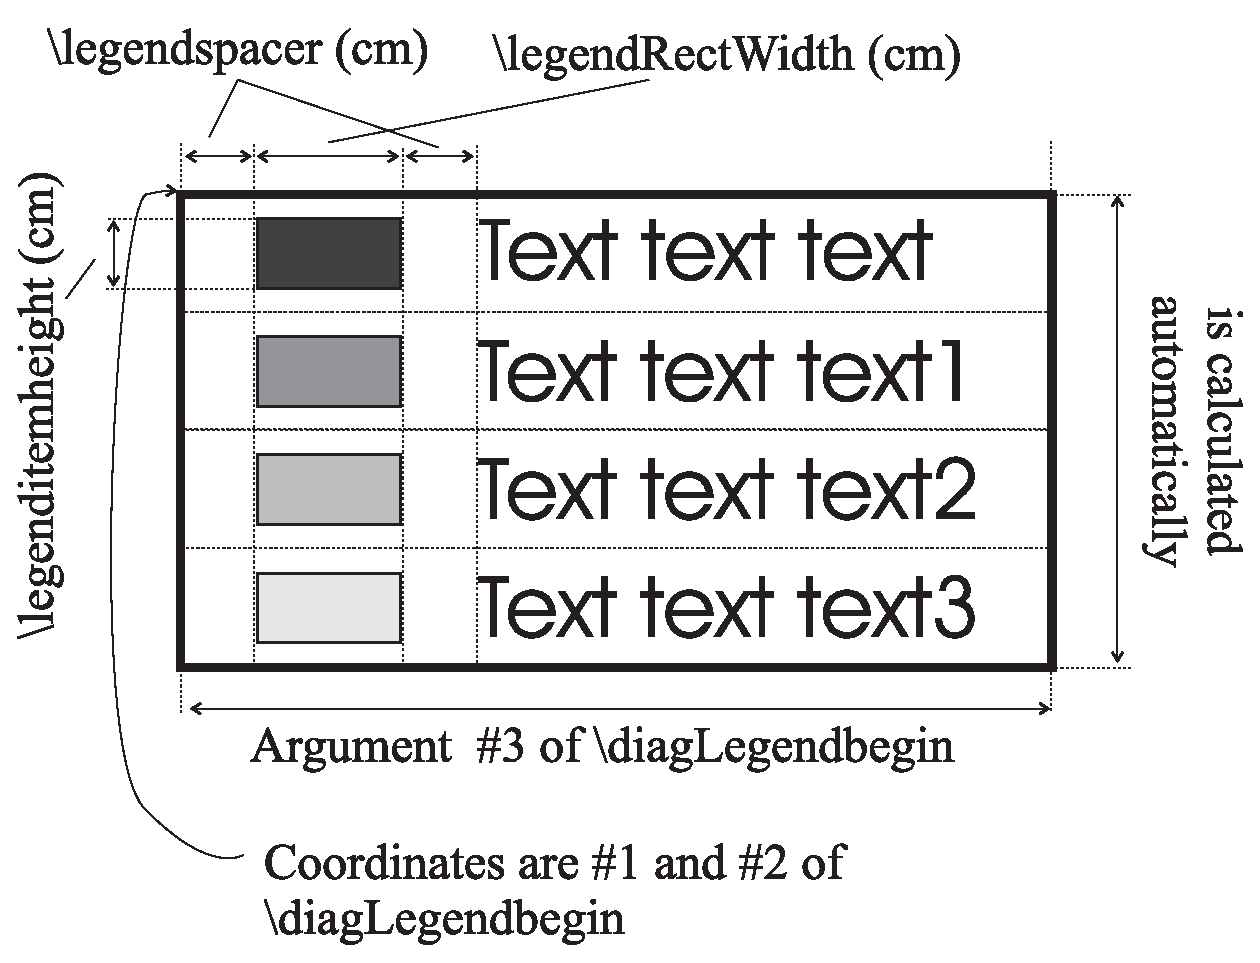
\includegraphics[scale=0.5]{figs/diagleg.eps}
\caption{\label{fig:5} Legend-related parameters}
\end{figure}

Some properties of the legend can be changed using \\
\verb+\diagLegendoptions{framefillcolor}{framelinecolor}{framelinewidth}+
\index{Commands!Legend!diagLegendoptions}
command.

\subsection{Groups of items \label{sec:2.3}}
I can imagine that you need more than just bars with figures. Let me
introduce one more feature: grouping of items as in \figref{fig:6}.
\begin{figure}[t]\centering
  \renewcommand{\betweenticks}{50}
\bardiagrambegin{12.5}{200}{2cm}{1}{2.5}{0.9cm}{0.05cm}
    \drawlevellines
    \baritem{1998}{123}{red}
        \subbaritem{}{118}{blue}
    \baritem{1999}{126}{red}
        \subbaritem{}{119}{blue}
    \baritem{2000}{144}{red}
        \subbaritem{}{148}{blue}
    \baritem{2001}{176}{red}
        \subbaritem{}{170}{blue}
    \baritem{2002}{128}{red}
        \subbaritem{}{134}{blue}  
    \diagLegendbegin{1}{190}{3.2}
      \diagLegenditem{Women}{red}
      \diagLegenditem{Men}{blue}
    \diagLegendend
\bardiagramend{{\large Year}}{{\large Income}}


\caption{\label{fig:6} Grouped items}
\end{figure}
This grouping is done using\\
\verb+\subbaritem{caption}{value}{color}+\index{Commands!subbaritem}. \\
So, a piece of code like
\begin{verbatim}
    \baritem{1998}{123}{red}
        \subbaritem{}{118}{blue}
\end{verbatim}
will produce \emph{two} bars next to each other.
You can go further and make groups of 3, 4, etc bars. In this way 
\begin{verbatim}
    \baritem{1998}{123}{red}
        \subbaritem{}{118}{blue}
        \subbaritem{}{108}{green}
\end{verbatim}
would produce group of 3 bars.

The ``bad news'' about \figref{fig:6} is that the labels (year) 
are not centered anymore. To correct the situation, just issue the command
\verb+\barspergroup{2}+ \index{Commands!barspergroup}
just after the beginning of the chart. It commands
the \bardiag\ to place the label assuming each group of items to be 2 bars wide.

Another way of grouping items is put them on top of each other
as in \figref{fig:7}, where, actually, two these approaches are combined. 
The above explained \verb+\barspergroup+ trick is used here too.
\begin{figure}[ht]\centering
  \renewcommand{\betweenticks}{50}
\bardiagrambegin{12.5}{210}{2cm}{1}{2.5}{0.8cm}{0.04cm}
    \barspergroup{2}
    \drawlevellines
    \baritem{1998}{23}{lightred}
      \subtopbaritem{}{100}{red}
    \subbaritem{}{28}{lightblue}
      \subtopbaritem{}{90}{blue}
    %
    \baritem{1999}{37}{lightred}
      \subtopbaritem{}{89}{red}
    \subbaritem{}{38}{lightblue}
      \subtopbaritem{}{81}{blue}
    %
    \baritem{2000}{43}{lightred}
      \subtopbaritem{}{101}{red}
    \subbaritem{}{52}{lightblue}
      \subtopbaritem{}{96}{blue}
    %
    \baritem{2001}{83}{lightred}
      \subtopbaritem{}{93}{red}
    \subbaritem{}{92}{lightblue}
      \subtopbaritem{}{78}{blue}
    %
    \baritem{2002}{64}{lightred}
      \subtopbaritem{}{64}{red}
    \subbaritem{}{70}{lightblue}
      \subtopbaritem{}{64}{blue}
    %
    \diagLegendbegin{0}{222}{7.3}
      \diagLegenditem{\it Women older than 30}{red}
      \diagLegenditem{\it Women younger than 30}{lightred}
      \diagLegenditem{\it Men older than 30}{blue}
      \diagLegenditem{\it Men younger than 30}{lightblue}
    \diagLegendend
\bardiagramend{{\large Year}}{{\large Income}}


\caption{\label{fig:7} Grouped items}
\end{figure}
The corresponding source code is shown below:
\lstinputlisting{figs/examp3.tex}
The command \verb+\subtopbaritem+ \index{Commands!subtopbaritem} has
the same arguments as other ``baritem'' commands and produces a bar on
top of the previous ``baritem'', which can be \verb+\baritem+, 
\verb+\subbaritem+ or even \verb+\subtopbaritem+.

\subsection{Making a 3D frame \label{sec:2.4}}
Frame can be done 3-dimensional by using the switch
\verb+\frameTD+. Its default value is 0, however, using\\
\verb+\renewcommand{\frameTD}{1}+
\index{Switches!frameTD}
\\
a 3D frame can be forced. To control the 3D effect, parameters
\verb+\tdx+ and \verb+\tdy+ are used [section~\ref{sec:3.5}].
Here, \figref{fig:8a}, is an example of the same diagram as in
\figref{fig:1} but with a 3D frame
%
\begin{figure}[!ht]
\renewcommand{\betweenticks}{50}
\subfigure[3D frame]{\label{fig:8a}
  \renewcommand{\frameTD}{1}
  \centering
    \bardiagrambegin{7.8}{210}{2cm}{1}{1.5}{0.7cm}{0.02cm}
      \drawlevellines
      \baritem{1998}{120}{green}
      \baritem{1999}{123}{red}
      \baritem{2000}{147}{yellow}
      \baritem{2001}{176}{green}
      \baritem{2002}{132}{red} 
      %
      \diagLegendbegin{0}{200}{3.8}
        \diagLegenditem{\it Legend}{red}
      \diagLegendend
  \bardiagramend{{\large Year}}{{\large Income}}
}
\subfigure[3D items]{\label{fig:8b}
 \renewcommand{\frameTD}{0}
 \renewcommand{\ActiveBarPrimitive}{\barTDRect}
   \bardiagrambegin{7.8}{210}{2cm}{1}{1.5}{0.7cm}{0.02cm}
      \drawlevellines
      \baritem{1998}{120}{green}
      \baritem{1999}{123}{red}
      \baritem{2000}{147}{yellow}
      \baritem{2001}{176}{green}
      \baritem{2002}{132}{red} 
      %
      \diagLegendbegin{0}{200}{3.8}
        \diagLegenditem{\it Legend}{red}
      \diagLegendend
  \bardiagramend{{\large Year}}{{\large Income}}
}
\caption{\label{fig:8} 3D effects}
\end{figure}

\subsection{Adding shadow to the legend \label{sec:2.5}}
You can force the legend to have a shadow by\\
\verb+\newcommand{\legendShadow}{1}+\index{Switches!legendShadow}.\\
However, if you use a 3D frame this will be done automatically.

\subsection{Changing the item-bar shape \label{sec:2.6}}
The \bard package provides also 3D item-bar shapes: rectangular 3d and
cylindrical. In fact, all the ``bar-item'' commands, such as
\verb+\XXXbaritem+, call the
\verb+\ActiveBarPrimitive+ command to draw ``a bar''. This means that
you can provide your own shapes [section \ref{sec:3.3}]. 

Concerning the shapes, provided by \bard: \figref{fig:8b} is an
example of\\ \verb+\renewcommand{\ActiveBarPrimitive}{\barTDrect}+
\index{Shape of an item-bar}\index{Shape of an item-bar!barTDrect}
command.
The default value \index{Shape of an item-bar!default}, \verb+\barRect+,
\index{Shape of an item-bar!barRect} produces a flat rectangle and 
\verb+\barCylinder+\index{Shape of an item-bar!barCylinder} a cylinder.
All these shapes can be grouped, etc, exactly in the same way as flat
rectangular bars.

The package provides: \verb+\barRect+, \verb+\barTDRect+,\verb+\barCylinder+.
Some additional shapes are discussed in \texttt{bardiag2.ps}.

\subsection{Adding error margins (``whiskers'')}
Adding ``whisker'' is simple! Just issue 
\verb+\barerrormargins{dYdown}{dYup}+ command after
the corresponding
\verb+\baritem+ or \verb+\subbaritem+\footnote{Unfortunately, 
it will not work with \texttt{subtopbaritem}.}.
\begin{lstlisting}{}
    \baritem{1998}{123}{gray} \barerror{25}
    \subbaritem{}{118}{lightgray} \barerrormargins{35}{15}
\end{lstlisting}
%
If you need symmetric whisker, use \verb+\barerror{dY}+ instead.
The properties of the ``whisker''-line are controlled by two parameters:\\ 
(i) \verb+\barerrorterm+ which defines the terminators. Default is 
\verb+\newcommand{\barerrorterm}{*-|}+, as in \figref{fig:er}\\
(ii) \verb+barerrorstyle+ can change the color, thickness, etc; use 
\verb+\newpsstyle+ to redefine it. Default: 
\verb+\newpsstyle{barerrorstyle}{linewidth=2pt,linecolor=black}+.

Everything said above holds for ``horizontal'' diagrams (\texttt{bardiag1.ps})
as well.

\begin{figure}[t]\centering
  %\renewcommand{\bdorientation}{\bdhor}
  \renewcommand{\placenumber}{\bottom}
  \renewcommand\numbercolor{\black\bf}
  \newcommand{\lecol}{gray}
\newcommand{\ricol}{lightgray}
\renewcommand{\betweenticks}{50}
\bardiagrambegin{12.5}{200}{1cm}{1}{2.5}{0.9cm}{0.05cm}
    \drawlevellines
    \barspergroup{2}
    \renewcommand{\barlabelangle}{0}
    \baritem{1998}{123}{\lecol} \barerror{25}
        \subbaritem{}{118}{\ricol} \barerrormargins{35}{15}
    \baritem{1999}{126}{\lecol} \barerror{20}
        \subbaritem{}{119}{\ricol} \barerrormargins{35}{32}
    \baritem{2000}{144}{\lecol} \barerror{24}
        \subbaritem{}{148}{\ricol} \barerror{30}
    \baritem{2001}{176}{\lecol} \barerror{22}
        \subbaritem{}{170}{\ricol} \barerror{25}
    \baritem{2002}{128}{\lecol} \barerror{20}
        \subbaritem{}{134}{\ricol}  \barerror{30} 
    \diagLegendbegin{1}{190}{3.2} 
      \diagLegenditem{Women}{\lecol}
      \diagLegenditem{Men}{\ricol}
    \diagLegendend
\bardiagramend{{\large Year}}{{\large Income}}


\caption{\label{fig:er} Grouped items and ``whiskers''}
\end{figure}

%\lstinputlisting{figs/examp2er.tex}
\subsection{Pattern fillings and black-and-white documents}
In many cases one cannot use any colors, except grayscale: not so many
publications are printed in color. So, it would be handy to use patterns 
to fill the bar-items. This is possible, because \verb+\baritem+
and friends take also an optional argument: style. In fact, the default one is
\verb+fillstyle=solid+ to get solid filled rectangles. In fact, one can call\\
\verb+\baritem[fillstyle=vlines*]{xxx}{nnn}{gray}+\\ 
to produce a dashed bar. To
get more info about fill styles, look into the \pac{pstricks} documentation:
e.g.  \pac{psr-usr2.ps}, pp. 27--28. 
Three of the relevant styles are: \verb+vlines*+, \verb+hlines*+, and
\verb+crosshatch*+. Also parameters like \verb+hatchwidth+, \verb+hatchsep+,
\verb+hatchcolor+, \verb+hatchangle+ can be used. Both\\
\verb+\baritem[fillstyle=vlines*,hatchsep=8pt,hatchangle=30]{xxx}{nnn}{gray}+\\
and\\
\verb+\newpsstyle{myfill}{fillstyle=vlines*,hatchsep=8pt,hatchangle=30}+\\
\verb+\baritem[style=myfill]{xxx}{nnn}{gray}+\\
are acceptable and produce the same.
\begin{figure}[t]\centering
  %\renewcommand{\bdorientation}{\bdhor}
  \renewcommand{\placenumber}{\bottom}
  \renewcommand\numbercolor{\black\bf}
  \renewcommand{\betweenticks}{100}
\renewcommand{\shownumbers}{0}

\definecolor{gA}{gray}{0.5}
\definecolor{gB}{gray}{0.7}
\definecolor{gC}{gray}{0.9}

\newpsstyle{diagframestyle}{linewidth=2pt,linecolor=black}
\newpsstyle{stA}{linestyle=solid,hatchsep=6pt,fillstyle=vlines*}
\newpsstyle{stB}{linestyle=solid,hatchsep=6pt,fillstyle=hlines*}
\newpsstyle{stC}{linestyle=solid,hatchsep=6pt,fillstyle=crosshatch*}

\bardiagrambegin{17.3}{1000}{0.5cm}{1.5}{6}{0.5cm}{0.01cm}
       \newpsstyle{levellinestyle}{linewidth=0.5pt,linecolor=gray,linestyle=dashed}
       \renewcommand{\barlabelangle}{0}
       
       \barspergroup{3}
       
       \drawlevellines
       \baritem[style=stA]{Here}{161}{gA}
         \subtopbaritem[style=stA]{}{250}{gB}
         \subtopbaritem[style=stA]{}{150}{gC}
	\subbaritem[style=stB]{}{381}{gA}
         \subtopbaritem[style=stB]{}{200}{gB}
         \subtopbaritem[style=stB]{}{150}{gC}
	\subbaritem[style=stC]{}{281}{gA}
         \subtopbaritem[style=stC]{}{200}{gB}
         \subtopbaritem[style=stC]{}{50}{gC}
       %
       \baritem[style=stA]{There}{221}{gA}
         \subtopbaritem[style=stA]{}{150}{gB}
         \subtopbaritem[style=stA]{}{130}{gC}
	\subbaritem[style=stB]{}{281}{gA}
         \subtopbaritem[style=stB]{}{300}{gB}
         \subtopbaritem[style=stB]{}{150}{gC}
	\subbaritem[style=stC]{}{121}{gA}
         \subtopbaritem[style=stC]{}{211}{gB}
         \subtopbaritem[style=stC]{}{350}{gC}
       %
       \baritem[style=stA]{Elsewhere}{432}{gA}
         \subtopbaritem[style=stA]{}{50}{gB}
         \subtopbaritem[style=stA]{}{230}{gC}
	\subbaritem[style=stB]{}{201}{gA}
         \subtopbaritem[style=stB]{}{130}{gB}
         \subtopbaritem[style=stB]{}{90}{gC}
	\subbaritem[style=stC]{}{191}{gA}
         \subtopbaritem[style=stC]{}{88}{gB}
         \subtopbaritem[style=stC]{}{222}{gC}
       %
       % we can call
       \diagLegendoptions{white}{white}{0pt}
       % to produce a legend without a frame
%
       \diagLegendbegin{0.5}{980}{3.5}
         \diagLegenditem[style=stA]{19.12.2002}{white}
         \diagLegenditem[style=stB]{06.05.2003}{white}
	 \diagLegenditem[style=stC]{01.02.2004}{white}
       \diagLegendend
       %
       \diagLegendbegin{7}{980}{3.5}
         \diagLegenditem{first try}{gA}
         \diagLegenditem{second try}{gB}
	 \diagLegenditem{third try}{gC}
       \diagLegendend
\bardiagramend{}{\large Number of smth}

\caption{\label{fig:cr} Using optional style argument of ``baritem'' and
                        ``diagLegenditem''}
\end{figure}
A comprehensive example to study is presented in \figref{fig:cr}:
\lstinputlisting{figs/exampcr.tex}

As shown in this example, the same technique applies to \verb+\diagLegenditem+.

Note, not all ``bar shapes'' will make use of the style you supply: e.g.,
there is no use in pattern-filled 3D cylinders because they look flat.
All the bar-primitives do accept the style option. It should always work well
for \verb+\barRect+ and \verb+\barArrowRect+. In the case of \verb+\barTDRect+ 
you can try to play around
-- personally, I do not see much use of it. 
Such primitives as \verb+\barCylinder+,
\verb+\barGradRect+, \verb+\barGradMidRect+, \verb+\barGradCylinder+ will just
ignore this optional argument.


\subsection{Additional information \label{sec:2.7}}
Try to have a look at the examples, which can be found in the
\texttt{example} directory.
%
%#########################################
%
\clearpage
\mysection{A more sophisticated example \label{sec:3}}
See \figref{fig:9}. More examples can be found in \texttt{bardiag1.ps} and
\texttt{bardiag2.ps}. In \texttt{bardiag1.ps} it is also explained how 
to draw a ``horizontally'' oriented diagram.

\begin{figure}[!ht]\centering
  \def\onecol{red}
\def\onetopcol{blue}
\def\twocol{red}
\def\twotopcol{blue}
\def\threecol{red}
\def\threetopcol{blue}
%-------------------------------------------------------
%This is the way to redefine styles
% \newpsstyle{mytickstyle}{linewidth=1pt,linecolor=blue}
%
% Style of the foreground frame
\newpsstyle{diagframestyle}{linewidth=1pt,linecolor=black,fillcolor=white}
% Style of the background frame
\newpsstyle{diagbgframestyle}{linewidth=1pt,linecolor=black,fillcolor=yellow}

% Use 3D bars
\renewcommand{\ActiveBarPrimitive}{\barTDRect}
% Make frame 3D
\renewcommand{\frameTD}{1}

% Put ticks and levellines each 10 yunits
\renewcommand{\betweenticks}{10}

% Color of the numbers on the bar-items 
\renewcommand\numbercolor{\white\bf}
% Where to put the number. Can be \bottom,\belowtop,\overtop
\renewcommand{\placenumber}{\bottom}


% override the default \tdx and \tdy
\renewcommand{\tdx}{1.2} % depth of 3d
\renewcommand{\tdy}{6}

% Start the diagram
\bardiagrambegin{14}{100}{3cm}{1}{5}{0.8cm}{0.1cm}
% To draw ``years'' at 45 degrees 
\renewcommand{\barlabelangle}{45}
       \baritem{1990}{32}{\onecol}
          \subtopbaritem{}{40}{\onetopcol}
        \subbaritem{2000}{20}{\twocol}
          \subtopbaritem{}{30}{\twotopcol}
        \subbaritem{2010}{13}{\threecol}
          \subtopbaritem{}{50}{\threetopcol}
       %---
       \baritem{1990}{21}{\onecol}
          \subtopbaritem{}{60}{\onetopcol}
        \subbaritem{2000}{25}{\twocol} 
          \subtopbaritem{}{64}{\twotopcol}
        \subbaritem{2010}{58}{\threecol}  
          \subtopbaritem{}{32}{\threetopcol}
       %---
       \baritem{1990}{22}{\onecol}
          \subtopbaritem{}{19}{\onetopcol}
        \subbaritem{2000}{12}{\twocol}
          \subtopbaritem{}{18}{\twotopcol}
        \subbaritem{2010}{9}{\threecol} 
          \subtopbaritem{}{12}{\threetopcol}
\drawlevellines
    % Legend
    %  Let's make the background white
    %  and gray frame-line of 0.5pt
    \diagLegendoptions{white}{gray}{0.5pt}
    % 
    \renewcommand{\legendShadowColor}{darkyellow}
    %
    \diagLegendbegin{10.3}{89}{3}
      \diagLegenditem{girls}{\onecol}
      \diagLegenditem{boys}{\onetopcol}
    \diagLegendend
    % End of the legend
\bardiagramend{\parbox{11cm}{\vspace{-1.5cm}\hspace{-1cm}
   \begin{tabular}{p{3.2cm}p{4.0cm}p{3.2cm}}
      \centering Alpha's & \centering Beta's & \centering Gamma's
   \end{tabular}
   \\[0.4cm]
   \centering \large Year}}
  {\large Graduated (\%)}

\caption{\label{fig:9} A more sophisticated example. See
   \texttt{bardiag2.ps} for the source code.}
\end{figure}

\subsection{Frame properties \label{sec:3.1}}
\begin{enumerate}
\item \verb+\bardiagrambegin{#1}{#2}{#3}{#4}{#5}{#6}{#7}+ 
      \index{Commands!bardiagrambegin}
      see \figref{fig:2}
   \begin{itemize}
       \item[\#1] diagram height (number)
       \item[\#2] diagram width (number)
       \item[\#3] bottom height (length, use \texttt{cm},
                  \texttt{in},\ldots)
       \item[\#4] bar width (number)
       \item[\#5] distance between (groups) of bars
       \item[\#6] x unit length (\texttt{cm},
                  \texttt{in},\ldots)
       \item[\#7] y unit length (\texttt{cm},
                  \texttt{in},\ldots)
   \end{itemize}    
\item \verb+\bardiagramend{#1}{#2}+ \index{Commands!bardiagramend}
   \begin{itemize}
       \item[\#1] X label (text, things like \verb+\bf,\it+, color can
         be used)
       \item[\#2] Y label (the same)
   \end{itemize} 
\item Parameters to be changed using \verb+\renewcommand+:
  \begin{itemize}    
     \item   \verb+\frameTD+ \index{Switches!frameTD}
       (default 0) can 1 or 0; makes the frame
       3D or 2D
  \end{itemize}
\item Parameters to be changed using \verb+\setlengt+:
   \begin{itemize}
     \item \verb+\leftshift+ \index{Lengths!leftshift}
       (default \verb+\ticklength++2mm) is the
       distance between the first bar and the frame left edge
     \item \verb+\textoffset+  \index{Lengths!textoffset}
       (default -0.2mm) see \figref{fig:2}
     \item \verb+\captionoffset+ \index{Lengths!captionoffset}
       (default 1.5cm) see \figref{fig:2}
   \end{itemize}
\item Styles, use \verb+\newpsstyle+ to change
   \begin{itemize}
     \item \verb+diagframestyle+ \index{Styles!diagframestyle} 
       is style of a 2D frame; defined as\\
       \verb+\newpsstyle{diagframestyle}{linewidth=1pt,linecolor=black,fillstyle=none}+
     \item \verb+diagTDframestyle+  \index{Styles!diagTDframestyle}
       is style of the foreground of a 3D frame;\\
       \verb+\newpsstyle{diagTDframestyle}+\\
       \verb+       {linewidth=1pt,linecolor=black,fillstyle=none}+
     \item \verb+diagbgframestyle+ \index{Styles!diagbgframestyle}
       is style of the background of a 3D frame;\\
       \verb+\newpsstyle{diagbgframestyle}+\\
       \verb+           {linewidth=1pt,linecolor=black,fillcolor=frameBGgray}+\\
       Also the definition \verb+\definecolor{frameBGgray}{gray}{0.9}+
       is used.
   \end{itemize}
\end{enumerate}

% - - - - - - - 
\subsection{Level lines and ticks \label{sec:3.2}}
 Both are produced by the \verb+\drawlevellines+ command. It can be
 issued at \emph{any} point inside a diagram.
\begin{enumerate}
\item Parameters to be changed using \verb+\renewcommand+:
      \begin{itemize} 
        \item \verb+\betweenticks+ \index{Parameters!betweenticks}
          is the distance between
          ticks/level lines in units of \verb+yunit+, so no \texttt{cm}
          allowed 
        \item \verb+\MAXnumberofticks+ \index{Parameters!MAXnumberofticks}
          (default is 20) is the maximal
          number of ticks/level lines allowed. If \verb+\betweenticks+
          is so small that the number of ticks exceeds
          \verb+\MAXnumberofticks+, the latter will be used (\bard
          will complain however, so a warning will be issued). 
        \item \verb+\barlabelangle+ \index{Parameters!barlabelangle}
          determines the angle of labels to be written below the
          bars. It has to be changed \emph{after}
          \verb+\bardiagrambegin+
          is called, otherwise it will automatically be set to 90
          degrees for vertical bars and 0 for horizontal ones.
        \item \verb+\ticklabelangle+ is almost the same as 
          \index{Parameters!ticklabelangle}
          \texttt{barlabelangle} but for the tick labels. It can
          be set at any point, not only after the beginnig of a diagram.
      \end{itemize}
\item Parameters to be changed using \verb+\setlengt+:
        \begin{itemize} 
        \item \verb+\ticklength+ \index{Lengths!ticklength}
          (default 2mm) is length of a tick on the y-axis
        \item \verb+\lefttextoffset+ \index{Lengths!lefttextoffset}
              (default \verb+\leftshift++2mm) 
              see \figref{fig:2}
      \end{itemize}
\item Styles, use \verb+\newpsstyle+ to change
   \begin{itemize}
     \item \verb+tickstyle+ \index{Styles!tickstyle} 
       is the tick style; defined as\\ 
       \verb+\newpsstyle{tickstyle}{linewidth=1pt,linecolor=black}+
     \item \verb+levellinestyle+ \index{Styles!levellinestyle}
       is the level line style;\\
       \verb+\newpsstyle{levellinestyle}{linewidth=0.2pt,linecolor=blue}+
   \end{itemize}
\end{enumerate}

% - - - - - - - 
\subsection{Bars \label{sec:3.3}}
\begin{enumerate}
\item \verb+\baritem{name}{value}{color}+ \index{Commands!baritem}
  is used to show a
  ``bar''. Actually it calls\\ \verb+\ActiveBarPrimitive+ 
  to draw the ``bar''.
\item \verb+\subbaritem{}{}{}+ \index{Commands!subbaritem}
  is used to produce a bar next to the
  previous bar (on the right hand side) without any space in between.
\item \verb+\subtopbaritem{}{}{}+ \index{Commands!subtopbaritem}
  is used to produce a bar on top of
  the previous bar.
\item \verb+\ActiveBarPrimitive+ \index{Commands!ActiveBarPrimitive}
  is used by all ``baritem'' commands
  to draw something that represents a bar. In fact, the
  \verb+\ActiveBarPrimitive+ is just a ``pointer'' to a command, which
  will really do the job. \bard provides 3 such commands:
  \verb+\barRect+,  \index{Commands!barRect}\index{Switches!barRect}
  \verb+\barTDRect+, \index{Commands!barTDRect}\index{Switches!barTDRect}
  and \verb+\barCylinder+.  \index{Commands!barCylinder}\index{Switches!barCylinder}
  Use,
  e.g., \verb+\renewcommand{\ActiveBarPrimitive}{\barCylinder}+ to
  draw cylinders instead of default rectangles. You can write your own
  ``shape'' (say \verb+\mybar+) 
  and put it somewhere in the preamble of the document or in
  the \texttt{bardiag.cfg}\index{bardiag.cfg} file and then point
  \verb+\ActiveBarPrimitive+ to it [see \texttt{bardiag.cfg} in
  \texttt{example} directory]. The \verb+\mybar+
  should accept 5 arguments: (\#1,\#2) and (\#3,\#4) are coordinates
  of the bottom-left and upper-right corners and \#5 is the color.
  In the \texttt{bardiag.cfg} file, which can be found, e.g., in the
  examples directory, a couple of ``alternative'' shapes are defined. 
  Examples can be found in \texttt{altdiag.tex} and in the appendix 
  (see file \texttt{bardiag2.tex} or \texttt{bardiag2.ps}).
%
\item Parameters to be changed using \verb+\renewcommand+:
      \begin{itemize} 
        \item \verb+\shownumbers+  \index{Switches!shownumbers}
          \index{Numbers!shownumbers}
          (default 1) use 1 to show 
          and 0 to hide the numbers on item-bars
        \item \verb+\numbercolor+ \index{Parameters!numbercolor}
         \index{Numbers!numbercolor}
         (default \verb+\black\bf+) is the
          color of these numbers
        \item \verb+\placenumber+ \index{Switches!placenumber}
          \index{Numbers!placenumber}
          (default \verb+\belowtop+)
          determines where on the bar put the number; can be
          \verb+\belowtop+, \verb+ \overtop+, \verb+\bottom+
          \index{Parameters!placenumber!belowtop}
          \index{Parameters!placenumber!overtop}
          \index{Parameters!placenumber!bottom}
      \end{itemize}
%
\item Parameters to be changed using \verb+\setlengt+:
        \begin{itemize} 
        \item \verb+\numberoffset+ \index{Lengths!numberoffset}
          (default \verb+2\textoffset+) is
          offset of the number on a bar
          from the top (if \verb+\overtop+ or \verb+\belowtop+
          are used) or the bottom (if \verb+\bottom+ is used)
      \end{itemize}
\end{enumerate}

% - - - - - - 
\subsection{Legend \label{sec:3.4}}
\begin{enumerate}
\item \verb+\diagLegendbegin{}{}{}+ \index{Commands!Legend!diagLegendbegin}
  begins a legend. 
  (\#1,\#2) is a coordinate of the top-left corner, \#3 is the width
  of the bounding box (all in units, not is \texttt{cm} or \texttt{in}).
  It is assumed
  that diagram is started above. Each diagram can have any number of
  legends. 
\item \verb+\diagLegendend+ \index{Commands!Legend!diagLegendend}
  ends a legend. It is needed to draw a shadow.
\item \verb+\diagLegendoptions{}{}{}+ \index{Commands!Legend!diagLegendoptions}
  is used to change the legend
  background color  (\#1), frame line color (\#2), and frame line
  width (\#3).
\item \verb+\diagLegenditem{}{}+ \index{Commands!Legend!diagLegenditem}
  adds one item to the legend: \#1 is
  text, \#2 is color. A rectangle of the color \#2 will be drawn and
  the text \#1 printed next to it.
\item Parameters to be changed using \verb+\renewcommand+:
      \begin{itemize} 
        \item \verb+\legendShadow+ \index{Switches!legendShadow}
          (default 0) - can be 1(=show the
          legend shadow) or 0(=do not); is switched on or off
          automatically if the frame is 3D or 2D, but can be adjusted
          by the final user as well
        \item \verb+\legendShadowColor+ \index{Parameters!legendShadowColor}
          (default \verb+legShCol+,
          where \verb+\definecolor{legShCol}{gray}{.5}+)       
      \end{itemize}
%
\item Parameters to be changed using \verb+\setlength+:
      \begin{itemize} 
        \item \verb+\legenditemheight+ \index{Lengths!legenditemheight}
              (default 7mm) - see \figref{fig:5}
        \item \verb+\legendspacer+  \index{Lengths!legendspacer}
              (default 3mm) - see \figref{fig:5}
        \item \verb+\legendRectWidth+ \index{Lengths!legendRectWidth}
          (default 6mm) is width of the
          colored rectangle; see \figref{fig:5}
        \item \verb+\legendRectHeight+ \index{Lengths!legendRectHeight}
         (default 4mm) is height of the
          colored rectangle; see \figref{fig:5}
      \end{itemize}
\item Styles (to be changed by \verb+\newpsstyle+)
      \begin{itemize} 
        \item \verb+diagLegenditemstyle+ \index{Styles!diagLegenditemstyle}
              is a style for the rectangle,
              which appears left to the legend text; default\\
              \verb+fillstyle=solid,fillcolor=white,linecolor=white+
          is not supposed to be changed directly (use
          \texttt{diagLegendoptions}), although it's up to you.
        \item+diagLegendframetyle+ \index{Styles!diagLegendframetyle}
              is a style for the bounding box
              around the legend; default\\
              \verb+fillstyle=none,linecolor=black,linewidth=0.5pt+
          is not supposed to be changed directly (use
          \texttt{diagLegendoptions}), although it's up to you.
      \end{itemize}
\end{enumerate}

%- - - - 
\subsection{3D effects \label{sec:3.5}}
\begin{figure}[!h]\centering
  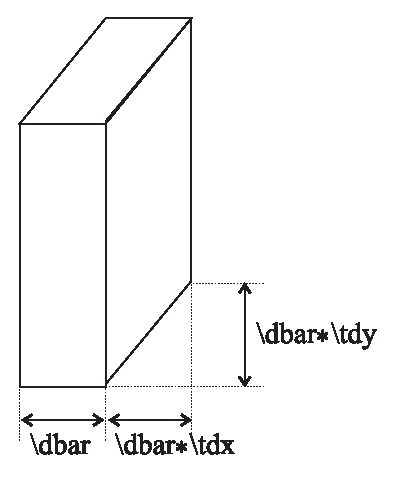
\includegraphics[scale=0.7]{figs/tddiag.eps}
\caption{\label{fig:3d}``Depth'' of the 3D-effect}
\end{figure}
 ``Depth'' of the 3D effect is controlled by \verb+\tdx+ and
 \verb+\tdy+ parameters 
 \index{Parameters!tdx (3D depth)} \index{Parameters!tdy (3D depth)}
 (default - \verb+\tdx+=0.4 and \verb+\tdy+ is 5\% of the diagram height). 
 They determine the
 ``depth'' in units of the bar width \verb+\dbar+, \figref{fig:3d}.
 Use \verb+\renewcommand+ to change them. Note, that the \verb+\renewcommand+
 is to be issued \emph{after} the \verb+\begindiagram+ statement.
%#########################################


\printindex

\end{document}
